\tikzstyle{vertex interior}=[fill,minimum size=0.80cm,circle,
    inner sep=0pt,outer sep=0.2pt,color=red!20]
\tikzstyle{vertex border}=[draw,thin,minimum size=0.80cm,circle,
    inner sep=0pt,outer sep=0.2pt,color=black]
\tikzstyle{vertex hidden}=[draw,minimum size=0.80cm,circle,
    inner sep=0pt,outer sep=0.2pt, color=gray, text=gray]
\tikzstyle{subvertex}=[color=gray]

\tikzstyle{bigvertex interior}=[fill=red!20]
\tikzstyle{bigvertex border}=[]

\tikzstyle{transition}=[semithick]

\newcommand{\vertex}[3][]{
    \node[vertex interior] at (#2) (#3) {};
    \node[vertex border,#1] at (#3) {\small #3};
}

\newcommand{\numberedvertex}[4][]{
    \node[vertex interior] at (#2) (#3) {};
    \node[vertex border,#1] at (#3) {\small #4};
}

\newcommand{\vertexnolabel}[3][]{
    \node[vertex interior] at (#2) (#3) {};
    \node[vertex border,#1] at (#3) {};
}

\newcommand{\wildcard}{\ensuremath{\star}}

% Usage: \if\blank{#1}...\else...\fi
\catcode`\@=11 % as in plain.tex
\long\def\blank#1{\bl@nk#1@@..\bl@nk}%
\long\def\bl@nk#1#2@#3#4\bl@nk{#3#4}
\catcode`\@=12

\long\def\test#1{\begingroup \toks0{[#1]}%
    \newlinechar`\/\message{/\the\toks0:
        \if\blank{#1}EMPTY\else NOT empty\fi%
    }\endgroup}

\newcommand{\hiddenvertex}[1]{
    \if \blank{#1}
    \else
        \node[vertex hidden] at (#1) {#1};
    \fi
}

\newcommand{\hiddenvertices}[4]{
    \hiddenvertex{#1}
    \hiddenvertex{#2}
    \hiddenvertex{#3}
    \hiddenvertex{#4}
}

\newcommand{\verticalvertexborder}[3][]{
    \draw[bigvertex border, #1] (#2.west) arc(180:0:2.9mm) -- 
        (#3.east) arc(0:-180:2.9mm) -- (#2.west);
}

\newcommand{\verticalvertex}[5][]{
    \draw[bigvertex interior, #1] (#2.west) arc(180:0:2.9mm) -- 
        (#3.east) arc(0:-180:2.9mm) -- (#2.west);
	\hiddenvertices{#2}{#3}{#4}{#5}
	\verticalvertexborder{#2}{#3}
}

\newcommand{\verticalgoalvertex}{\verticalvertex[color=green!40]}

\newcommand{\horizontalvertexborder}[3][]{
    \draw[bigvertex border, #1] (#2.south) arc(-90:-270:2.9mm) -- 
        (#3.north) arc(90:-90:2.9mm) -- (#2.south);
}

\newcommand{\horizontalvertex}[3][]{
    \draw[bigvertex interior, #1] (#2.south) arc(-90:-270:2.9mm) -- 
        (#3.north) arc(90:-90:2.9mm) -- (#2.south);
	\hiddenvertices{#2}{#3}{}{}
	\horizontalvertexborder{#2}{#3}
}

\newcommand{\trianglevertexleftborder}[4][]{
    \draw[bigvertex border,#1] (#2.south west) arc(-135:-225:2.9mm) -- 
        (#3.north west) arc(135:0:2.9mm) -- 
        (#4.east) arc(0:-135:2.9mm) -- 
        (#2.south west);
}

\newcommand{\trianglevertexleft}[5][]{    
    \draw[bigvertex interior, #1] (#2.south west) arc(-135:-225:2.9mm) -- 
        (#3.north west) arc(135:0:2.9mm) -- 
        (#4.east) arc(0:-135:2.9mm) -- 
        (#2.south west); 
	\hiddenvertices{#2}{#3}{#4}{#5}
	\trianglevertexleftborder{#2}{#3}{#4}
}

\newcommand{\trianglevertexrightborder}[4][]{
    \draw[bigvertex border, #1] (#2.south east) arc(-45:45:2.9mm) -- 
        (#3.north east) arc(45:180:2.9mm) -- 
        (#4.west) arc(180:315:2.9mm) -- 
        (#2.south east);
}

\newcommand{\trianglevertexright}[5][]{   
    \draw[bigvertex interior, #1] (#2.south east) arc(-45:45:2.9mm) -- 
        (#3.north east) arc(45:180:2.9mm) -- 
        (#4.west) arc(180:315:2.9mm) -- 
        (#2.south east); 
	\hiddenvertices{#2}{#3}{#4}{#5}
	\trianglevertexrightborder{#2}{#3}{#4}
}

\newcommand{\squarevertexborder}[5][]{
    \draw[bigvertex border] (#2.west) arc(180:90:2.9mm) -- 
        (#3.north) arc(90:0:2.9mm) -- 
        (#4.east) arc(0:-90:2.9mm) -- 
        (#5.south) arc(-90:-180:2.9mm) -- 
        (#2.west);
}

\newcommand{\squarevertex}[5][]{    
    \draw[bigvertex interior, #1] (#2.west) arc(180:90:2.9mm) -- 
        (#3.north) arc(90:0:2.9mm) -- 
        (#4.east) arc(0:-90:2.9mm) -- 
        (#5.south) arc(-90:-180:2.9mm) -- 
        (#2.west); 
	\hiddenvertices{#2}{#3}{#4}{#5}
	\squarevertexborder{#2}{#3}{#4}{#5}
}

\newcommand{\gravisvertexborder}[3][]{
    \draw[bigvertex border, #1] (#2.south west) arc(225:45:2.9mm) -- 
        (#3.north east) arc(45:-135:2.9mm) -- 
        (#2.south west);
}

\newcommand{\gravisvertex}[3][]{    
    \draw[bigvertex interior,#1] (#2.south west) arc(225:45:2.9mm) -- 
        (#3.north east) arc(45:-135:2.9mm) -- 
        (#2.south west); 
	\hiddenvertices{#2}{#3}{}{}
	\gravisvertexborder{#2}{#3}
}

\newcommand{\akutvertexborder}[3][]{
    \draw[bigvertex border, #1] (#2.north west) arc(135:-45:2.9mm) -- 
        (#3.south east) arc(-45:-225:2.9mm) -- 
        (#2.north west);
}

\newcommand{\akutvertex}[3][]{    
    \draw[bigvertex interior,#1] (#2.north west) arc(135:-45:2.9mm) -- 
        (#3.south east) arc(-45:-225:2.9mm) -- 
        (#2.north west); 
	\hiddenvertices{#2}{#3}{}{}
	\akutvertexborder{#2}{#3}
}

\newcommand{\goalvertex}[3][]{
    \node[vertex interior,color=green!40] at (#2) (#3) {};
    \node[vertex border,#1] at (#3) {\small #3};
}

\newcommand{\numberedgoalvertex}[4][]{
    \node[vertex interior,color=green!40] at (#2) (#3) {};
    \node[vertex border,#1] at (#3) {\small #4};
}

\newcommand{\goalvertexnolabel}[3][]{
    \node[vertex interior,color=green!40] at (#2) (#3) {};
    \node[vertex border,#1] at (#3) {};
}

\newcommand{\transition}[5][]{\draw[<->,>=stealth,transition,#1] (#2)--(#3);}

\newcommand{\circletransition}{140:1.25mm}
\newcommand{\selftransition}[2][0:0mm]{
    \draw[->,>=stealth,transition] (#2) +(#1) arc(-45:225:1.5mm);}

\newcommand{\picfulltransitiongraphbase}[2]{%
  \begin{tikzpicture}[scale=1.4]
    #1{0,0}{LRR}
    %
    \draw[transition,->,>=stealth](-0.6,0) -- (LRR);
    %
    #1{1,0}{LLL}
    #1{1,1}{LLR}
    #1{1,-1}{LRL}
    %
    #1{2,1.5}{ALR}
    #1{2,0.5}{ALL}
    #1{2,-0.5}{BLL}
    #1{2,-1.5}{BRL}
    %
    #1{3,1.5}{ARL}
    #1{3,0.5}{ARR}
    #1{3,-0.5}{BRR}
    #1{3,-1.5}{BLR}
    %
    #2{4,0}{RRR}
    #2{4,1}{RRL}
    #2{4,-1}{RLR}
    %
    #2{5,0}{RLL}
    %
    \transition{LLL}{LRL}{move(A,R)}{move(A,L)}
    \transition{LLL}{LLR}{move(B,R)}{move(B,L)}
    \transition{LRL}{LRR}{move(B,R)}{move(B,L)}
    \transition{LLR}{LRR}{move(A,R)}{move(A,L)}
    %
    \transition{LLL}{ALL}{pick(A,L)}{drop(A,L)}
    \transition{LLL}{BLL}{pick(B,L)}{drop(B,L)}
    \transition{LLR}{ALR}{pick(A,L)}{drop(A,L)}
    \transition{LRL}{BRL}{pick(B,L)}{drop(B,L)}
    \transition{ALL}{ALR}{move(A,R)}{move(A,L)}
    \transition{BLL}{BRL}{move(B,R)}{move(B,L)}
    %
    \transition{ALR}{ARR}{move(A,R)}{move(A,L)}
    \transition{ALL}{ARL}{move(A,R)}{move(A,L)}
    \transition{BRL}{BRR}{move(B,R)}{move(B,L)}
    \transition{BLL}{BLR}{move(B,R)}{move(B,L)}
    %
    \transition{RRR}{ARR}{pick(A,R)}{drop(A,R)}
    \transition{RRR}{BRR}{pick(B,R)}{drop(B,R)}
    \transition{RRL}{ARL}{pick(A,R)}{drop(A,R)}
    \transition{RLR}{BLR}{pick(B,R)}{drop(B,R)}
    \transition{ARR}{ARL}{move(A,L)}{move(A,R)}
    \transition{BRR}{BLR}{move(B,L)}{move(B,R)}
    %
    \transition{RRR}{RLR}{move(A,L)}{move(A,R)}
    \transition{RRR}{RRL}{move(B,L)}{move(B,R)}
    \transition{RLR}{RLL}{move(B,L)}{move(B,R)}
    \transition{RRL}{RLL}{move(A,L)}{move(A,R)}
  \end{tikzpicture}%
}

\newcommand{\picfulltransitiongraph}{%
  \picfulltransitiongraphbase{\vertex}{\goalvertex}}

\newcommand{\picfulltransitiongraphnolabels}{%
  \picfulltransitiongraphbase{\vertexnolabel}{\goalvertexnolabel}}

\newcommand{\picperfectabstraction}{%
  \begin{tikzpicture}[scale=1.4]
    \vertex[text=gray]{0,0}{LRR}
    %
    \draw[transition,->,>=stealth](-0.6,0) -- (LRR);
    %
    \vertex{1,1}{LLR}
    \vertex{1,0}{LLL}
    \vertex{1,-1}{LRL}
    \verticalvertex{LLR}{LRL}{LLL}{}
    %
    \vertex{2,1.5}{ALR}
    \vertex{2,0.5}{ALL}
    \vertex{2,-0.5}{BLL}
    \vertex{2,-1.5}{BRL}
    \verticalvertex{ALR}{BRL}{ALL}{BLL}
    %
    \vertex{3,1.5}{ARL}
    \vertex{3,0.5}{ARR}
    \vertex{3,-0.5}{BRR}
    \vertex{3,-1.5}{BLR}
    \verticalvertex{ARL}{BLR}{ARR}{BRR}
    %
    %
    \vertex{4,0}{RRR}
    \vertex{4,1}{RRL}
    \vertex{4,-1}{RLR}
    \vertex{5,0}{RLL}
    \trianglevertexright[fill=green!40]{RLL}{RRL}{RLR}{RRR}
    %
    \transition{LLL}{LRR}{}{}
    %
    \transition{LLL}{LLL-|ALL.west}{}{}
    %
    \transition{LLL-|ALL.east}{RRR-|ARL.west}{}{}
    %
    \transition{RRR}{RRR-|ARL.east}{}{}
    %
    \selftransition[\circletransition]{LLR.north east}
    \selftransition[\circletransition]{ALR.north east}
    \selftransition[\circletransition]{ARL.north east}
    \selftransition[\circletransition]{RRL.north east}
  \end{tikzpicture}%
}

\newcommand{\piconestateabstraction}{%
  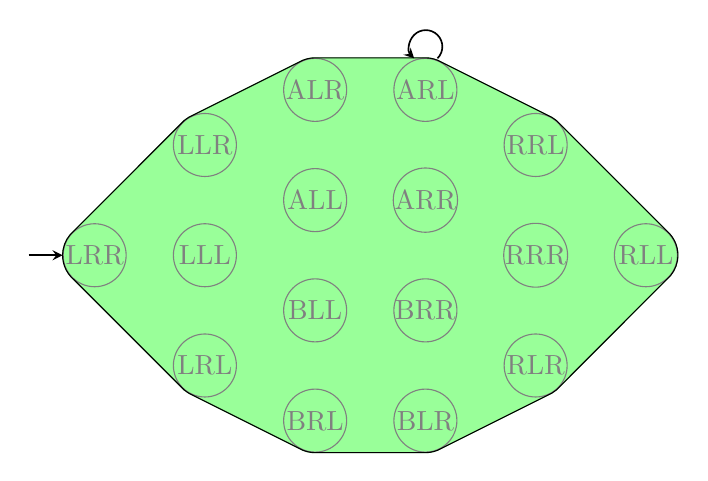
\begin{tikzpicture}[scale=1.4]
    \vertex[text=gray]{0,0}{LRR}
    %
    \draw[transition,->,>=stealth](-0.6,0) -- (LRR);
    %
    \vertex{1,1}{LLR}
    \vertex{1,0}{LLL}
    \vertex{1,-1}{LRL}
    \vertex{2,1.5}{ALR}
    \vertex{2,0.5}{ALL}
    \vertex{2,-0.5}{BLL}
    \vertex{2,-1.5}{BRL}
    \vertex{3,1.5}{ARL}
    \vertex{3,0.5}{ARR}
    \vertex{3,-0.5}{BRR}
    \vertex{3,-1.5}{BLR}
    \vertex{4,0}{RRR}
    \vertex{4,1}{RRL}
    \vertex{4,-1}{RLR}
    \vertex{5,0}{RLL}
	
    \draw[bigvertex interior,color=green!40] (LRR.230) arc(-130:-230:2.9mm)
    -- (LLR.140) arc(-220:-240:2.9mm)
    -- (ALR.120) arc(-240:-270:2.9mm) -- (ARL.north) arc(90:60:2.9mm)
    -- (RRL.60) arc (-300:-320:2.9mm) -- (RLL.50) arc(50:-50:2.9mm)
	-- (RLR.320) arc (-40:-60:2.9mm) -- (BLR.300) arc (-60:-90:2.9mm)
	-- (BRL.south) arc (-90:-120:2.9mm) -- (LRL.240) arc (-120:-140:2.9mm)
	-- (LRR.230);
	\hiddenvertices{LRR}{LLR}{LLL}{LRL}
	\hiddenvertices{ALR}{ALL}{BLL}{BRL}
	\hiddenvertices{ARL}{ARR}{BRR}{BLR}
	\hiddenvertices{RRR}{RRL}{RLR}{RLL}
    \draw[bigvertex border] (LRR.230) arc(-130:-230:2.9mm)
    -- (LLR.140) arc(-220:-240:2.9mm)
    -- (ALR.120) arc(-240:-270:2.9mm) -- (ARL.north) arc(90:60:2.9mm)
    -- (RRL.60) arc (-300:-320:2.9mm) -- (RLL.50) arc(50:-50:2.9mm)
	-- (RLR.320) arc (-40:-60:2.9mm) -- (BLR.300) arc (-60:-90:2.9mm)
	-- (BRL.south) arc (-90:-120:2.9mm) -- (LRL.240) arc (-120:-140:2.9mm)
	-- (LRR.230);
	
    \selftransition[\circletransition]{ARL.north east}
  \end{tikzpicture}%
}

\newcommand{\picexampleabstraction}[1][\verticalvertex]{%
  \begin{tikzpicture}[scale=1.4]
    \vertex[text=gray]{0,0}{LRR}
    %
    \draw[transition,->,>=stealth](-0.6,0) -- (LRR);
    %
    \vertex{1,1}{LLR}
    \vertex{1,0}{LLL}
    \vertex{1,-1}{LRL}
    #1{LLR}{LRL}{LLL}{}
    %
    \vertex{2,1.5}{ALR}
    \vertex{3,1.5}{ARL}
    \vertex{2,0.5}{ALL}
    \vertex{3,0.5}{ARR}
    \vertex{2,-0.5}{BLL}
    \vertex{2,-1.5}{BRL}
    \vertex{3,-0.5}{BRR}
    \vertex{3,-1.5}{BLR}
    \squarevertex{ALR}{ARL}{BLR}{BRL}
	\hiddenvertices{ALL}{ARR}{BLL}{BRR}
    %
    \vertex{4,0}{RRR}
    \vertex{4,1}{RRL}
    \vertex{4,-1}{RLR}
    \vertex{5,0}{RLL}
    \trianglevertexright[fill=green!40]{RLL}{RRL}{RLR}{RRR}
    %
    \draw[transition,->,>=stealth](-0.6,0) -- (LRR);
    %
    \transition{LRR}{LLL}{}{}
    \transition{LLL}{LLL-|ALL.west}{}{}
    \transition{RRR}{RRR-|ARL.east}{}{}
    %
    \selftransition[\circletransition]{LLR.north east}
    \selftransition[\circletransition]{RRL.north east}
    \selftransition[0:6mm]{ALR.north}
  \end{tikzpicture}
}

\newcommand{\picprojectionpackage}{%
  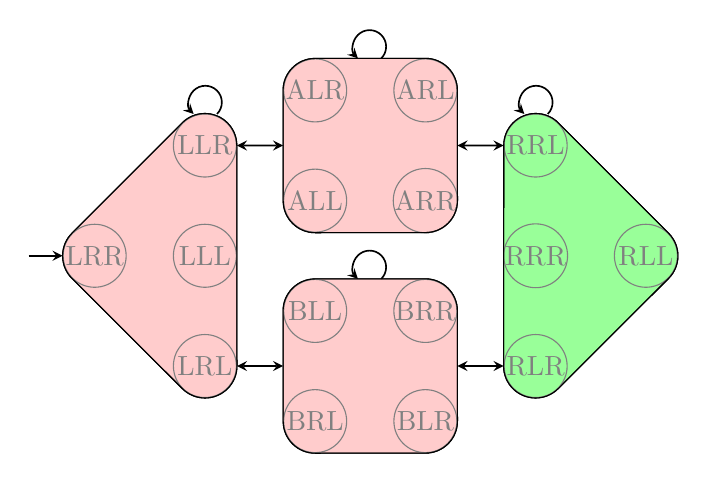
\begin{tikzpicture}[scale=1.4]
    \vertex{0,0}{LRR}
    \vertex{1,0}{LLL}
    \vertex{1,1}{LLR}
    \vertex{1,-1}{LRL}
    \trianglevertexleft{LRR}{LLR}{LRL}{LLL}
    %
    \vertex{2,1.5}{ALR}
    \vertex{3,1.5}{ARL}
    \vertex{2,0.5}{ALL}
    \vertex{3,0.5}{ARR}
    \squarevertex{ALR}{ARL}{ARR}{ALL}
    %
    \vertex{2,-0.5}{BLL}
    \vertex{2,-1.5}{BRL}
    \vertex{3,-0.5}{BRR}
    \vertex{3,-1.5}{BLR}
    \squarevertex{BLL}{BRR}{BLR}{BRL}
    %
    \vertex{4,0}{RRR}
    \vertex{4,1}{RRL}
    \vertex{4,-1}{RLR}
    \vertex{5,0}{RLL}
    \trianglevertexright[fill=green!40]{RLL}{RRL}{RLR}{RRR}
    %
    \draw[transition,->,>=stealth](-0.6,0) -- (LRR);
    %
    \transition{LLR}{LLR-|ALR.west}{}{}
    \transition{LRL}{LRL-|BRL.west}{}{}
    \transition{RRL}{RRL-|ARL.east}{}{}
    \transition{RLR}{RLR-|ARL.east}{}{}
    \selftransition[\circletransition]{LLR.north east}
    \selftransition[\circletransition]{RRL.north east}
    \selftransition[0:6mm]{ALR.north}
    \selftransition[0:6mm]{BLL.north}
  \end{tikzpicture}
}

\newcommand{\picprojectionpackagetruck}{
  \begin{tikzpicture}[scale=1.4]
    \vertex{0,0}{LRR}
    \vertex{1,-1}{LRL}
    \gravisvertex{LRR}{LRL}
    %
    \vertex{1,0}{LLL}
    \vertex{1,1}{LLR}
    \verticalvertex{LLR}{LLL}{}{}
    %
    \vertex{2,1.5}{ALR}
    \vertex{2,0.5}{ALL}
    \verticalvertex{ALR}{ALL}{}{}
    %
    \vertex{3,1.5}{ARL}
    \vertex{3,0.5}{ARR}
    \verticalvertex{ARL}{ARR}{}{}
    %
    \only<beamer:1|handout:0>{
      \vertex{3,-1.5}{BLR}
      \vertex{2,-0.5}{BLL}
      \vertex{3,-0.5}{BRR}
      \vertex{2,-1.5}{BRL}
      \gravisvertex{BLL}{BLR}
      \akutvertex{BRR}{BRL}
    }%
    \only<2>{
      \vertex{3,-1.5}{BRR}
      \vertex{2,-0.5}{BLL}
      \vertex{3,-0.5}{BLR}
      \vertex{2,-1.5}{BRL}
      \horizontalvertex{BLL}{BLR}
      \horizontalvertex{BRL}{BRR}
    }%
    %
    \vertex{4,0}{RRR}
    \vertex{4,1}{RRL}
    \verticalvertex[fill=green!40]{RRL}{RRR}{}{}
    %
    \vertex{4,-1}{RLR}
    \vertex{5,0}{RLL}
    \akutvertex[fill=green!40]{RLL}{RLR}
    %
    \draw[transition,->,>=stealth](-0.6,0) -- (LRR);
    \transition{intersection of LRR.north east--LRL.north east and LRR.east--LLL.west}
      {LLL.north-|LLR.west}{}{}
    \transition{ALL.north west-|LLR.east}{LLR.east-|ALL.west}{}{}
    \transition{LLR.east-|ALL.east}{LLR.east-|ARR.west}{}{}
    \transition{LLR.east-|ARL.east}{ARR.north east-|RRL.west}{}{}
    \transition{RRR.north-|RRR.east}
      {intersection of RLL.north west--RLR.north west and RLL.west--RRR.east}{}{}
    %
    \transition{LLL.north-|LLL.east}{BLL}{}{}
    \transition{LRL}{BRL}{}{}
    \only<beamer:1|handout:0>{\transition{BRR}{RRR.west|-RRR.north}{}{}}
    \only<2>{\transition{BRR.north east}{RRR.south west}{}{}}
    \transition{BLR}{RLR}{}{}
    \only<beamer:1|handout:0>{\transition{BRL.south east}{BLR.south west}{}{}}
    \only<2>{\transition{BLL.south-|BLL.east}{BRL.north-|BRL.east}{}{}}
    \selftransition[\circletransition]{LRR.north east}
    \selftransition[\circletransition]{LLR.north east}
    \selftransition[\circletransition]{ALR.north east}
    \selftransition[\circletransition]{ARL.north east}
    \selftransition[\circletransition]{RRL.north east}
    \selftransition[\circletransition]{RLL.north east}
    \only<beamer:1|handout:0>{
      \selftransition[\circletransition]{BLL.north east}
      \selftransition[\circletransition]{BRR.north east}
    }%
    \only<2>{
      \selftransition[1:8mm]{BLL.north}
      \selftransition[1:8mm]{BRL.north}
    }%
  \end{tikzpicture}%
}

\newcommand{\picrefinement}{%
  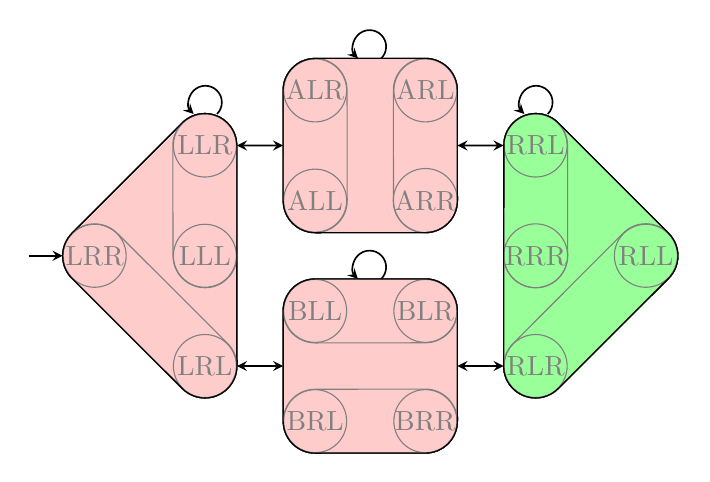
\begin{tikzpicture}[scale=1.4]
    \vertex{0,0}{LRR}
    \vertex{1,0}{LLL}
    \vertex{1,1}{LLR}
    \vertex{1,-1}{LRL}
    \trianglevertexleft{LRR}{LLR}{LRL}{LLL}
    \gravisvertexborder[subvertex]{LRR}{LRL}
    \verticalvertexborder[subvertex]{LLR}{LLL}
    \trianglevertexleftborder{LRR}{LLR}{LRL}{LLL}
    %
    \vertex{2,1.5}{ALR}
    \vertex{3,1.5}{ARL}
    \vertex{2,0.5}{ALL}
    \vertex{3,0.5}{ARR}
    \squarevertex{ALR}{ARL}{ARR}{ALL}
    \verticalvertexborder[subvertex]{ALR}{ALL}
    \verticalvertexborder[subvertex]{ARL}{ARR}
    \squarevertexborder{ALR}{ARL}{ARR}{ALL}
    %
    \vertex{2,-0.5}{BLL}
    \vertex{2,-1.5}{BRL}
    \vertex{3,-0.5}{BLR}
    \vertex{3,-1.5}{BRR}
    \squarevertex{BLL}{BLR}{BRR}{BRL}
    \horizontalvertexborder[subvertex]{BLL}{BLR}
    \horizontalvertexborder[subvertex]{BRL}{BRR}
    \squarevertexborder{BLL}{BLR}{BRR}{BRL}
    %
    \vertex{4,0}{RRR}
    \vertex{4,1}{RRL}
    \vertex{4,-1}{RLR}
    \vertex{5,0}{RLL}
    \trianglevertexright[fill=green!40]{RLL}{RRL}{RLR}{RRR}
    \verticalvertexborder[subvertex]{RRL}{RRR}
    \akutvertexborder[subvertex]{RLL}{RLR}
    \trianglevertexrightborder{RLL}{RRL}{RLR}{RRR}
	%
    \draw[transition,->,>=stealth](-0.6,0) -- (LRR);
    %
    \transition{LLR}{LLR-|ALR.west}{}{}
    \transition{LRL}{LRL-|BRL.west}{}{}
    \transition{RRL}{RRL-|ARL.east}{}{}
    \transition{RLR}{RLR-|ARL.east}{}{}
    \selftransition[\circletransition]{LLR.north east}
    \selftransition[\circletransition]{RRL.north east}
    \selftransition[0:6mm]{ALR.north}
    \selftransition[0:6mm]{BLL.north}
  \end{tikzpicture}
}


\newcommand{\pictwopackages}{%
  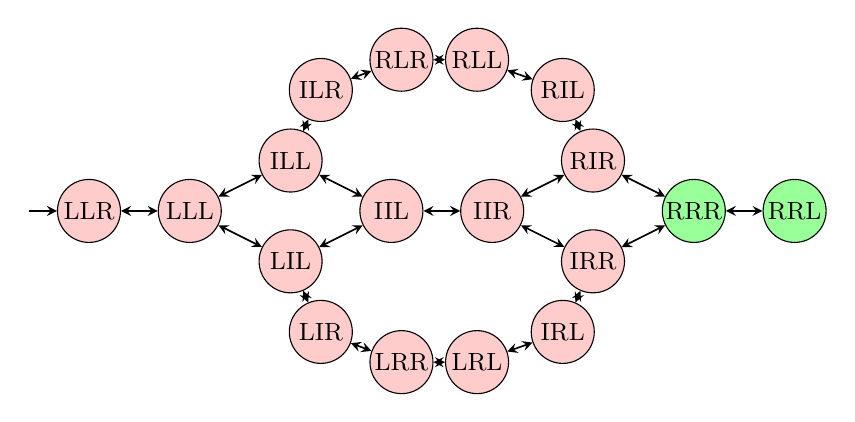
\begin{tikzpicture}[scale=1.28]
    \vertex{0,0}{LLR}
    \vertex{1,0}{LLL}
    \vertex{2,.5}{ILL}
    \vertex{2,-.5}{LIL}
    \vertex{3,0}{IIL}
    \vertex{4,0}{IIR}
    \vertex{5,.5}{RIR}
    \vertex{5,-.5}{IRR}
    \goalvertex{6,0}{RRR}
    \goalvertex{7,0}{RRL}
    \vertex{2.3,1.2}{ILR}
    \vertex{3.1,1.5}{RLR}
    \vertex{3.85,1.5}{RLL}
    \vertex{4.7,1.2}{RIL}
    \vertex{2.3,-1.2}{LIR}
    \vertex{3.1,-1.5}{LRR}
    \vertex{3.85,-1.5}{LRL}
    \vertex{4.7,-1.2}{IRL}

    \draw[transition,->,>=stealth](-0.6,0) -- (LLR);
    \transition{LLR}{LLL}{}{}
    \transition{LLL}{ILL}{}{}
    \transition{LLL}{LIL}{}{}
    \transition{ILL}{IIL}{}{}
    \transition{LIL}{IIL}{}{}
    \transition{IIL}{IIR}{}{}
    \transition{IIR}{RIR}{}{}
    \transition{IIR}{IRR}{}{}
    \transition{RIR}{RRR}{}{}
    \transition{IRR}{RRR}{}{}
    \transition{RRR}{RRL}{}{}
    \transition{ILL}{ILR}{}{}
    \transition{RLR}{ILR}{}{}
    \transition{RLR}{RLL}{}{}
    \transition{RIL}{RLL}{}{}
    \transition{RIL}{RIR}{}{}
    \transition{LIL}{LIR}{}{}
    \transition{LRR}{LIR}{}{}
    \transition{LRR}{LRL}{}{}
    \transition{LRL}{IRL}{}{}
    \transition{IRR}{IRL}{}{}
  \end{tikzpicture}
}

\newlength{\vertexround}
\setlength{\vertexround}{3.14mm}
\newcommand{\pictwopackagesabstractpacktwo}{%
  \begin{tikzpicture}[scale=1.28]
    \vertex{0,0}{LLR}
    \vertex{1,0}{LLL}
    \vertex{2,.5}{ILL}
    \vertex{2,-.5}{LIL}
    \vertex{3,0}{IIL}
    \vertex{4,0}{IIR}
    \vertex{5,.5}{RIR}
    \vertex{5,-.5}{IRR}
    \goalvertex{6,0}{RRR}
    \goalvertex{7,0}{RRL}
    \vertex{2.3,1.2}{ILR}
    \vertex{3.1,1.5}{RLR}
    \vertex{3.85,1.5}{RLL}
    \vertex{4.7,1.2}{RIL}
    \vertex{2.3,-1.2}{LIR}
    \vertex{3.1,-1.5}{LRR}
    \vertex{3.85,-1.5}{LRL}
    \vertex{4.7,-1.2}{IRL}
    
    \draw[bigvertex interior] (LLR.south) arc(-90:-240:\vertexround)
    -- (ILR.120) arc(120:100:\vertexround) 
	-- (RLR.110) arc (110:90:\vertexround)
    -- (RLL.north) arc(90:-60:\vertexround) -- (ILL.-60)
    -- (LLL.300) arc (-60:-90:\vertexround) -- (LLR.south);
	\hiddenvertices{LLR}{LLL}{ILL}{ILR}
	\hiddenvertices{RLR}{RLL}{}{}
    \draw[bigvertex border] (LLR.south) arc(-90:-240:\vertexround)
    -- (ILR.120) arc(120:100:\vertexround) 
	-- (RLR.120) arc (120:90:\vertexround)
    -- (RLL.north) arc(90:-60:\vertexround) -- (ILL.-60)
    -- (LLL.300) arc (-60:-90:\vertexround) -- (LLR.south);
    
    \draw[bigvertex interior] (LIR.310) arc(-50:-165:\vertexround)
    -- (LIL.200) arc(-160:-240:\vertexround) 
    -- (RIL.120) arc(120:10:\vertexround)
    -- (RIR.20) arc(20:-50:\vertexround)
    -- (LIR.310);
	\hiddenvertices{LIR}{LIL}{IIL}{IIR}
	\hiddenvertices{RIR}{RIL}{}{}
    \draw[bigvertex border] (LIR.310) arc(-50:-165:\vertexround)
    -- (LIL.200) arc(-160:-240:\vertexround) 
    -- (RIL.120) arc(120:10:\vertexround)
    -- (RIR.20) arc(20:-50:\vertexround)
    -- (LIR.310);

    \draw[bigvertex interior, color=green!40] (RRL.north) arc(90:-60:\vertexround)
    -- (IRL.-60) arc(-60:-80:\vertexround)
	-- (LRL.-70) arc (-70:-90:\vertexround)
    -- (LRR.south) arc(-90:-240:\vertexround) -- (IRR.120)
    -- (RRR.120) arc (120:90:\vertexround) -- (RRL.north);
	\hiddenvertices{LRR}{LRL}{IRL}{IRR}
	\hiddenvertices{RRR}{RRL}{}{}
    \draw[bigvertex border] (RRL.north) arc(90:-60:\vertexround)
    -- (IRL.-60) arc(-60:-80:\vertexround)
	-- (LRL.-70) arc (-70:-90:\vertexround)
    -- (LRR.south) arc(-90:-240:\vertexround) -- (IRR.120)
    -- (RRR.120) arc (120:90:\vertexround) -- (RRL.north);

    \draw[transition,->,>=stealth](-0.6,0) -- (LLR);
    \transition{ILL.-60}{intersection of LIL.-240 -- RIL.120 and ILR.180 -- LRR.180}{}{}
    \transition{IRR.120}{intersection of RIR.-50 -- LIR.310 and IRL.0 -- RLL.0}{}{}
    \selftransition[-.5mm:-3mm]{RRL.north}
    \selftransition[-.1mm:1mm]{RIL.north}
    \begin{scope}[yscale=-1]
      \selftransition[-.5mm:-3mm]{LLL.south}
    \end{scope}

    \only<all:5>{
      \transition[gray,->]{LLR}{LLL}{}{}
      \transition[gray,->]{LLL}{ILL}{}{}
      \transition[gray,->]{ILL}{IIL}{}{}
      \transition[gray,->]{IIL}{IIR}{}{}
      \transition[gray,->]{IIR}{RIR}{}{}
      \transition[gray,->]{RIR}{RRR}{}{}
    }
  \end{tikzpicture}
}

\newcommand{\pictwopackagesabstractpackone}{%
  \begin{tikzpicture}[scale=1.28]
    \vertex{0,0}{LLR}
    \vertex{1,0}{LLL}
    \vertex{2,.5}{ILL}
    \vertex{2,-.5}{LIL}
    \vertex{3,0}{IIL}
    \vertex{4,0}{IIR}
    \vertex{5,.5}{RIR}
    \vertex{5,-.5}{IRR}
    \goalvertex{6,0}{RRR}
    \goalvertex{7,0}{RRL}
    \vertex{2.3,1.2}{ILR}
    \vertex{3.1,1.5}{RLR}
    \vertex{3.85,1.5}{RLL}
    \vertex{4.7,1.2}{RIL}
    \vertex{2.3,-1.2}{LIR}
    \vertex{3.1,-1.5}{LRR}
    \vertex{3.85,-1.5}{LRL}
    \vertex{4.7,-1.2}{IRL}
    
    \draw[bigvertex interior] (LLR.north) arc(90:240:\vertexround)
    -- (LIR.-120) arc(-120:-100:\vertexround) 
    -- (LRR.-110) arc (-110:-90:\vertexround)
    -- (LRL.south) arc(-90:60:\vertexround) -- (LIL.60)
    -- (LLL.-300) arc (60:90:\vertexround) -- (LLR.north);
    \hiddenvertices{LLR}{LLL}{LIL}{LIR}
    \hiddenvertices{LRR}{LRL}{}{}
    \draw[bigvertex border] (LLR.north) arc(90:240:\vertexround)
    -- (LIR.-120) arc(-120:-100:\vertexround) 
    -- (LRR.-110) arc (-110:-90:\vertexround)
    -- (LRL.south) arc(-90:60:\vertexround) -- (LIL.60)
    -- (LLL.-300) arc (60:90:\vertexround) -- (LLR.north);
    
    \draw[bigvertex interior] (ILR.-310) arc(50:165:\vertexround)
    -- (ILL.-200) arc(160:240:\vertexround) 
    -- (IRL.-120) arc(-120:-10:\vertexround)
    -- (IRR.-20) arc(-20:50:\vertexround)
    -- (ILR.-310);
    \hiddenvertices{ILR}{ILL}{IIL}{IIR}
    \hiddenvertices{IRR}{IRL}{}{}
    \draw[bigvertex border] (ILR.-310) arc(50:165:\vertexround)
    -- (ILL.-200) arc(160:240:\vertexround) 
    -- (IRL.-120) arc(-120:-10:\vertexround)
    -- (IRR.-20) arc(-20:50:\vertexround)
    -- (ILR.-310);

    \draw[bigvertex interior, color=green!40] (RRL.south) arc(-90:60:\vertexround)
    -- (RIL.60) arc(60:80:\vertexround)
    -- (RLL.70) arc (70:90:\vertexround)
    -- (RLR.north) arc(90:240:\vertexround) -- (RIR.-120)
    -- (RRR.-120) arc (-120:-90:\vertexround) -- (RRL.south);
    \hiddenvertices{RLR}{RLL}{RIL}{RIR}
    \hiddenvertices{RRR}{RRL}{}{}
    \draw[bigvertex border] (RRL.south) arc(-90:60:\vertexround)
    -- (RIL.60) arc(60:80:\vertexround)
    -- (RLL.70) arc (70:90:\vertexround)
    -- (RLR.north) arc(90:240:\vertexround) -- (RIR.-120)
    -- (RRR.-120) arc (-120:-90:\vertexround) -- (RRL.south);

    \draw[transition,->,>=stealth](-0.6,0) -- (LLR);
    \transition{LIL.60}{intersection of ILL.240 -- IRL.240 and LIR.180 -- RLR.180}{}{}
    \transition{LIL.60}{intersection of ILL.240 -- IRL.-120 and LIR.-180 -- RLR.-180}{}{}
    \transition{RIR.-120}{intersection of IRR.50 -- ILR.-310 and RIL.0 -- LRL.0}{}{}
    \selftransition[-.5mm:-3mm]{LLL.north}
    \selftransition[-.1mm:1mm]{ILR.north}
    \begin{scope}[yscale=-1]
      \selftransition[-.5mm:-3mm]{RRL.south}
    \end{scope}

    \only<all:3>{
      \transition[gray,->]{LLR}{LLL}{}{}
      \transition[gray,->]{LLL}{ILL}{}{}
      \transition[gray,->]{ILL}{IIL}{}{}
      \transition[gray,->]{IIL}{IIR}{}{}
      \transition[gray,->]{IIR}{RIR}{}{}
      \transition[gray,->]{RIR}{RRR}{}{}
    }
  \end{tikzpicture}
}

\newcommand{\bendtransition}[6][]{\draw[->,>=stealth,transition,#1] (#2) edge [#6] node[above=-1mm,sloped,#5] {\scriptsize #4} (#3);}
\newcommand{\bendtransitionnolabel}[6][]{\draw[->,>=stealth,transition,#1] (#2) edge [#6] node[above=-1mm,sloped,#5] {} (#3);}
\newcommand{\picatomicprojectionpackage}{%
  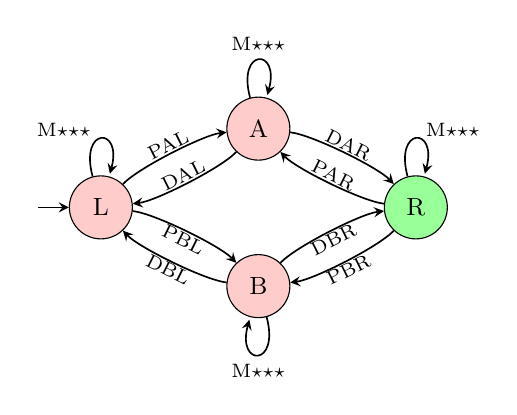
\begin{tikzpicture}[->,>=stealth,looseness=.5,bend angle=20]
       	\vertex{0,0}{L}
	\vertex{2,1}{A}
	\vertex{2,-1}{B}
	\goalvertex{4,0}{R}

	\draw[transition,->,>=stealth](-0.8,0) -- (L);
	\bendtransition{L}{L}{M{\wildcard}{\wildcard}{\wildcard}}{above left}{loop above}
	\bendtransition{L}{A}{PAL}{}{bend left}
	\bendtransition{A}{L}{DAL}{}{bend left}
	\bendtransition{A}{A}{M{\wildcard}{\wildcard}{\wildcard}}{above=1mm}{loop above}
	\bendtransition{A}{R}{DAR}{}{bend left}
	\bendtransition{R}{A}{PAR}{}{bend left}
	\bendtransition{R}{R}{M{\wildcard}{\wildcard}{\wildcard}}{above right}{loop above}
	\bendtransition{R}{B}{PBR}{below=-2mm}{bend left}
	\bendtransition{B}{R}{DBR}{below=-2mm}{bend left}
	\bendtransition{B}{B}{M{\wildcard}{\wildcard}{\wildcard}}{below=-1mm}{loop below}
	\bendtransition{B}{L}{DBL}{below=-2mm}{bend left}
	\bendtransition{L}{B}{PBL}{below=-2mm}{bend left}
  \end{tikzpicture}
}

\newcommand{\picatomicprojectionpackagenumberedstates}{%
  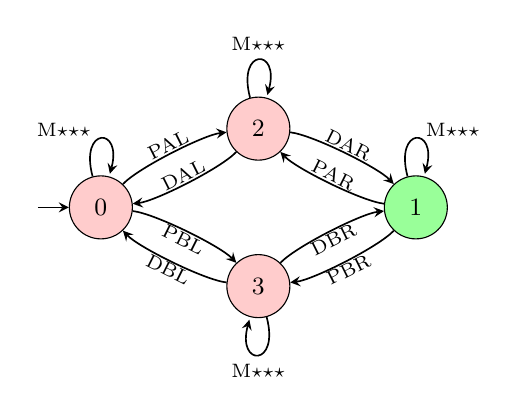
\begin{tikzpicture}[->,>=stealth,looseness=.5,bend angle=20]
        \numberedvertex{0,0}{L}{0}
	\numberedvertex{2,1}{A}{2}
	\numberedvertex{2,-1}{B}{3}
	\numberedgoalvertex{4,0}{R}{1}

	\draw[transition,->,>=stealth](-0.8,0) -- (L);
	\bendtransition{L}{L}{M{\wildcard}{\wildcard}{\wildcard}}{above left}{loop above}
	\bendtransition{L}{A}{PAL}{}{bend left}
	\bendtransition{A}{L}{DAL}{}{bend left}
	\bendtransition{A}{A}{M{\wildcard}{\wildcard}{\wildcard}}{above=1mm}{loop above}
	\bendtransition{A}{R}{DAR}{}{bend left}
	\bendtransition{R}{A}{PAR}{}{bend left}
	\bendtransition{R}{R}{M{\wildcard}{\wildcard}{\wildcard}}{above right}{loop above}
	\bendtransition{R}{B}{PBR}{below=-2mm}{bend left}
	\bendtransition{B}{R}{DBR}{below=-2mm}{bend left}
	\bendtransition{B}{B}{M{\wildcard}{\wildcard}{\wildcard}}{below=-1mm}{loop below}
	\bendtransition{B}{L}{DBL}{below=-2mm}{bend left}
	\bendtransition{L}{B}{PBL}{below=-2mm}{bend left}
  \end{tikzpicture}
}

\newcommand{\picatomicprojectiontrucka}{%
  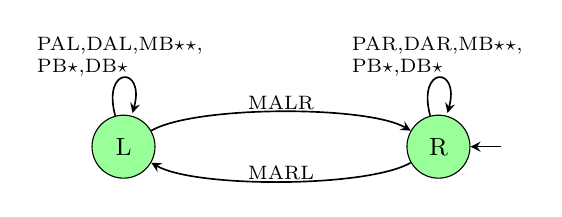
\begin{tikzpicture}[->,>=stealth,looseness=.5]
	\goalvertex{0,0}{L}
	\goalvertex{4,0}{R}

	\draw[transition,->,>=stealth](4.8,0) -- (R);
	\bendtransition{L}{L}{\parbox{22mm}{PAL,DAL,MB{\wildcard}{\wildcard},\\PB{\wildcard},DB{\wildcard}}}{above}{loop above}
	\bendtransition{L}{R}{MALR}{}{bend left}
	\bendtransition{R}{L}{MARL}{}{bend left}
	\bendtransition{R}{R}{\parbox{22mm}{PAR,DAR,MB{\wildcard}{\wildcard},\\PB{\wildcard},DB{\wildcard}}}{above}{loop above}
  \end{tikzpicture}
}

\newcommand{\picatomicprojectiontruckb}{%
  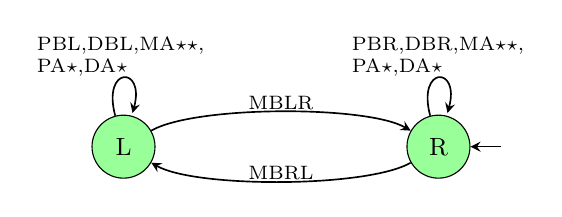
\begin{tikzpicture}[->,>=stealth,looseness=.5]
	\goalvertex{0,0}{L}
	\goalvertex{4,0}{R}

	\draw[transition,->,>=stealth](4.8,0) -- (R);
	\bendtransition{L}{L}{\parbox{22mm}{PBL,DBL,MA{\wildcard}{\wildcard},\\PA{\wildcard},DA{\wildcard}}}{above}{loop above}
	\bendtransition{L}{R}{MBLR}{}{bend left}
	\bendtransition{R}{L}{MBRL}{}{bend left}
	\bendtransition{R}{R}{\parbox{22mm}{PBR,DBR,MA{\wildcard}{\wildcard},\\PA{\wildcard},DA{\wildcard}}}{above}{loop above}
  \end{tikzpicture}
}

\newcommand{\picproductpackagetrucka}[1][]{%
  \begin{tikzpicture}[->,>=stealth,looseness=.5,bend angle=20,#1]
  	\vertex{0,0}{LL}
  	\vertex{2,0}{LR}
	\vertex{3,2}{AL}
	\vertex{5,2}{AR}
	\vertex{3,-2}{BL}
	\vertex{5,-2}{BR}
  	\goalvertex{6,0}{RL}
  	\goalvertex{8,0}{RR}
	
	\draw[transition,->,>=stealth](2.6,0.6) -- (LR);
	\bendtransition{LL}{LR}{MALR}{}{bend left}
	\bendtransition{LR}{LL}{MARL}{below=-2mm}{bend left}
	\bendtransition{AL}{AR}{MALR}{}{bend left}
	\bendtransition{AR}{AL}{MARL}{below=-2mm}{bend left}
	\bendtransition{BL}{BR}{MALR}{}{bend left}
	\bendtransition{BR}{BL}{MARL}{below=-2mm}{bend left}
	\bendtransition{RL}{RR}{MALR}{}{bend left}
	\bendtransition{RR}{RL}{MARL}{below=-2mm}{bend left}
	
	\bendtransition{LL}{AL}{PAL}{}{bend left=50}
	\bendtransition{AL}{LL}{DAL}{}{bend right}
	\bendtransition{AR}{RR}{DAR}{}{bend left=50}
	\bendtransition{RR}{AR}{PAR}{}{bend right}
	\bendtransition{RR}{BR}{PBR}{}{bend left=50}
	\bendtransition{BR}{RR}{DBR}{}{bend right}
	\bendtransition{BL}{LL}{DBL}{}{bend left=50}
	\bendtransition{LL}{BL}{PBL}{}{bend right}
	
	\bendtransition{LR}{BR}{PBL}{near start}{bend left=50}
	\bendtransition{BR}{LR}{DBL}{near end,below=-2mm}{bend right}
	\bendtransition{BL}{RL}{DBR}{near end}{bend left=50}
	\bendtransition{RL}{BL}{PBR}{near start,below=-2mm}{bend right}
	
	\bendtransition{LL}{LL}{MB{\wildcard}{\wildcard}}{above=2mm,pos=.9,sloped=false}{loop left}
	\bendtransition{RR}{RR}{MB{\wildcard}{\wildcard}}{above=2mm,pos=.1,sloped=false}{loop right}
	\bendtransition{AL}{AL}{MB{\wildcard}{\wildcard}}{}{loop above}
	\bendtransition{AR}{AR}{MB{\wildcard}{\wildcard}}{}{loop above}
	\bendtransition{LR}{LR}{MB{\wildcard}{\wildcard}}{}{loop above}
	\bendtransition{RL}{RL}{MB{\wildcard}{\wildcard}}{}{loop above}
	\bendtransition{BL}{BL}{MB{\wildcard}{\wildcard}}{below=-1mm}{loop below}
	\bendtransition{BR}{BR}{MB{\wildcard}{\wildcard}}{below=-1mm}{loop below}
  \end{tikzpicture}
}

\newcommand{\picproductpackagetruckanumberedstates}[1][]{%
  \begin{tikzpicture}[->,>=stealth,looseness=.5,bend angle=20,#1]
  	\numberedvertex{0,0}{LL}{0}
  	\numberedvertex{2,0}{LR}{1}
	\numberedvertex{3,2}{AL}{4}
	\numberedvertex{5,2}{AR}{5}
	\numberedvertex{3,-2}{BL}{6}
	\numberedvertex{5,-2}{BR}{7}
  	\numberedgoalvertex{6,0}{RL}{2}
  	\numberedgoalvertex{8,0}{RR}{3}
	
	\draw[transition,->,>=stealth](2.6,0.6) -- (LR);
	\bendtransition{LL}{LR}{MALR}{}{bend left}
	\bendtransition{LR}{LL}{MARL}{below=-2mm}{bend left}
	\bendtransition{AL}{AR}{MALR}{}{bend left}
	\bendtransition{AR}{AL}{MARL}{below=-2mm}{bend left}
	\bendtransition{BL}{BR}{MALR}{}{bend left}
	\bendtransition{BR}{BL}{MARL}{below=-2mm}{bend left}
	\bendtransition{RL}{RR}{MALR}{}{bend left}
	\bendtransition{RR}{RL}{MARL}{below=-2mm}{bend left}
	
	\bendtransition{LL}{AL}{PAL}{}{bend left=50}
	\bendtransition{AL}{LL}{DAL}{}{bend right}
	\bendtransition{AR}{RR}{DAR}{}{bend left=50}
	\bendtransition{RR}{AR}{PAR}{}{bend right}
	\bendtransition{RR}{BR}{PBR}{}{bend left=50}
	\bendtransition{BR}{RR}{DBR}{}{bend right}
	\bendtransition{BL}{LL}{DBL}{}{bend left=50}
	\bendtransition{LL}{BL}{PBL}{}{bend right}
	
	\bendtransition{LR}{BR}{PBL}{near start}{bend left=50}
	\bendtransition{BR}{LR}{DBL}{near end,below=-2mm}{bend right}
	\bendtransition{BL}{RL}{DBR}{near end}{bend left=50}
	\bendtransition{RL}{BL}{PBR}{near start,below=-2mm}{bend right}
	
	\bendtransition{LL}{LL}{MB{\wildcard}{\wildcard}}{above=2mm,pos=.9,sloped=false}{loop left}
	\bendtransition{RR}{RR}{MB{\wildcard}{\wildcard}}{above=2mm,pos=.1,sloped=false}{loop right}
	\bendtransition{AL}{AL}{MB{\wildcard}{\wildcard}}{}{loop above}
	\bendtransition{AR}{AR}{MB{\wildcard}{\wildcard}}{}{loop above}
	\bendtransition{LR}{LR}{MB{\wildcard}{\wildcard}}{}{loop above}
	\bendtransition{RL}{RL}{MB{\wildcard}{\wildcard}}{}{loop above}
	\bendtransition{BL}{BL}{MB{\wildcard}{\wildcard}}{below=-1mm}{loop below}
	\bendtransition{BR}{BR}{MB{\wildcard}{\wildcard}}{below=-1mm}{loop below}
  \end{tikzpicture}
}

\newcommand{\subpicatomicprojectionpackagesmall}{%
  \begin{scope}[->,>=stealth,looseness=.5,bend angle=20,scale=.7,transform shape]
	\vertex{0,0}{L}
	\vertex{2,1}{A}
	\vertex{2,-1}{B}
	\goalvertex{4,0}{R}

	\draw[transition,->,>=stealth](-0.8,0) -- (L);
	\bendtransition{L}{L}{M{\wildcard}{\wildcard}{\wildcard}}{above left}{loop above}
	\bendtransition{L}{A}{PAL}{}{bend left}
	\bendtransition{A}{L}{DAL}{}{bend left}
	\bendtransition{A}{A}{M{\wildcard}{\wildcard}{\wildcard}}{above=1mm}{loop above}
	\bendtransition{A}{R}{DAR}{}{bend left}
	\bendtransition{R}{A}{PAR}{}{bend left}
	\bendtransition{R}{R}{M{\wildcard}{\wildcard}{\wildcard}}{above right}{loop above}
	\bendtransition{R}{B}{PBR}{below=-2mm}{bend left}
	\bendtransition{B}{R}{DBR}{below=-2mm}{bend left}
	\bendtransition{B}{B}{M{\wildcard}{\wildcard}{\wildcard}}{below=-1mm}{loop below}
	\bendtransition{B}{L}{DBL}{below=-2mm}{bend left}
	\bendtransition{L}{B}{PBL}{below=-2mm}{bend left}
	
	\only<all:2>{\vertex[draw=red,thick]{2,1}{A}}
	\only<all:3>{\vertex[draw=red,thick]{0,0}{L}}
	\only<all:3>{\draw[transition,->,>=stealth,red](-0.8,0) -- (L);}
	\only<all:4>{\goalvertex[fill=green]{4,0}{R}}
	\only<all:5>{\bendtransition[red]{L}{A}{PAL}{}{bend left}}
	\only<all:6>{\bendtransition[red]{L}{L}{M{\wildcard}{\wildcard}{\wildcard}}{above left}{loop above}}
	\only<all:7>{\bendtransition[red]{L}{B}{PBL}{below=-2mm}{bend left}}
	\only<all:8>{\bendtransition[red]{A}{A}{M{\wildcard}{\wildcard}{\wildcard}}{above=1mm}{loop above}}
  \end{scope}
}

\newcommand{\subpicatomicprojectiontruckasmall}{%
  \begin{scope}[->,>=stealth,looseness=.5,scale=.7,transform shape]
	\goalvertex{0,0}{L}
	\goalvertex{4,0}{R}

	\draw[transition,->,>=stealth](4.8,0) -- (R);
	\bendtransition{L}{L}{\parbox{22mm}{PAL,DAL,MB{\wildcard}{\wildcard},\\PB{\wildcard},DB{\wildcard}}}{above}{loop above}
	\bendtransition{L}{R}{MALR}{}{bend left}
	\bendtransition{R}{L}{MARL}{}{bend left}
	\bendtransition{R}{R}{\parbox{22mm}{PAR,DAR,MB{\wildcard}{\wildcard},\\PB{\wildcard},DB{\wildcard}}}{above}{loop above}

	\only<all:2>{\goalvertex[draw=red,thick]{0,0}{L}}
	\only<all:3>{\goalvertex[draw=red,thick]{4,0}{R}}
	\only<all:3>{\draw[transition,->,>=stealth,red](4.8,0) -- (R);}
	\only<all:4>{\goalvertex[fill=green]{0,0}{L}}
	\only<all:5>{\bendtransition[red]{L}{L}{\parbox{22mm}{PAL\color{black},DAL,MB{\wildcard}{\wildcard},\\PB{\wildcard},DB{\wildcard}}}{above}{loop above}}
	\only<all:6>{\bendtransition[red]{L}{R}{MALR}{}{bend left}}
	\only<all:7>{\bendtransition[red]{R}{R}{\parbox{22mm}{\color{black}PAR,DAR,MB{\wildcard}{\wildcard},\\{\color{red}PB{\wildcard}},DB{\wildcard}}}{above}{loop above}}
	\only<all:8>{\bendtransition[red]{L}{L}{\parbox{22mm}{\color{black}PAL,DAL,{\color{red}MB{\wildcard}{\wildcard}},\\PB{\wildcard},DB{\wildcard}}}{above}{loop above}}
  \end{scope}
}

\newcommand{\subpicproductpackagetruckasmall}{%
  \begin{scope}[->,>=stealth,looseness=.5,,bend angle=20,scale=.7,transform shape]
  	\vertex{0,0}{LL}
  	\vertex{2,0}{LR}
	\vertex{3,2}{AL}
	\vertex{5,2}{AR}
	\vertex{3,-2}{BL}
	\vertex{5,-2}{BR}
  	\goalvertex{6,0}{RL}
  	\goalvertex{8,0}{RR}
	
	\draw[transition,->,>=stealth](2.6,0.6) -- (LR);
	\bendtransition{LL}{LR}{MALR}{}{bend left}
	\bendtransition{LR}{LL}{MARL}{below=-2mm}{bend left}
	\bendtransition{AL}{AR}{MALR}{}{bend left}
	\bendtransition{AR}{AL}{MARL}{below=-2mm}{bend left}
	\bendtransition{BL}{BR}{MALR}{}{bend left}
	\bendtransition{BR}{BL}{MARL}{below=-2mm}{bend left}
	\bendtransition{RL}{RR}{MALR}{}{bend left}
	\bendtransition{RR}{RL}{MARL}{below=-2mm}{bend left}
	
	\bendtransition{LL}{AL}{PAL}{}{bend left=50}
	\bendtransition{AL}{LL}{DAL}{}{bend right}
	\bendtransition{AR}{RR}{DAR}{}{bend left=50}
	\bendtransition{RR}{AR}{PAR}{}{bend right}
	\bendtransition{RR}{BR}{PBR}{}{bend left=50}
	\bendtransition{BR}{RR}{DBR}{}{bend right}
	\bendtransition{BL}{LL}{DBL}{}{bend left=50}
	\bendtransition{LL}{BL}{PBL}{}{bend right}
	
	\bendtransition{LR}{BR}{PBL}{near start}{bend left=50}
	\bendtransition{BR}{LR}{DBL}{near end,below=-2mm}{bend right}
	\bendtransition{BL}{RL}{DBR}{near end}{bend left=50}
	\bendtransition{RL}{BL}{PBR}{near start,below=-2mm}{bend right}
	
	\bendtransition{LL}{LL}{MB{\wildcard}{\wildcard}}{above=2mm,sloped=false,pos=.9}{loop left}
	\bendtransition{RR}{RR}{MB{\wildcard}{\wildcard}}{above=2mm,sloped=false,pos=.1}{loop right}
	\bendtransition{AL}{AL}{MB{\wildcard}{\wildcard}}{}{loop above}
	\bendtransition{AR}{AR}{MB{\wildcard}{\wildcard}}{}{loop above}
	\bendtransition{LR}{LR}{MB{\wildcard}{\wildcard}}{}{loop above}
	\bendtransition{RL}{RL}{MB{\wildcard}{\wildcard}}{}{loop above}
	\bendtransition{BL}{BL}{MB{\wildcard}{\wildcard}}{below=-1mm}{loop below}
	\bendtransition{BR}{BR}{MB{\wildcard}{\wildcard}}{below=-1mm}{loop below}
	
	\only<all:2>{\vertex[draw=red,thick]{3,2}{AL}}
	\only<all:3>{\vertex[draw=red,thick]{2,0}{LR}}
	\only<all:3>{\draw[transition,->,>=stealth,red](2.6,0.6) -- (LR);}
  	\only<all:4>{\goalvertex[fill=green]{6,0}{RL}}
	\only<all:5>{\bendtransition[red]{LL}{AL}{PAL}{}{bend left=50}}
	\only<all:6>{\bendtransition[red]{LL}{LR}{MALR}{}{bend left}}
	\only<all:7>{\bendtransition[red]{LR}{BR}{PBL}{near start}{bend left=50}}
	\only<all:8>{\bendtransition[red]{AL}{AL}{MB{\wildcard}{\wildcard}}{}{loop above}}
  \end{scope}
}

\newcommand{\picproductpackagetruckaillustration}{%
  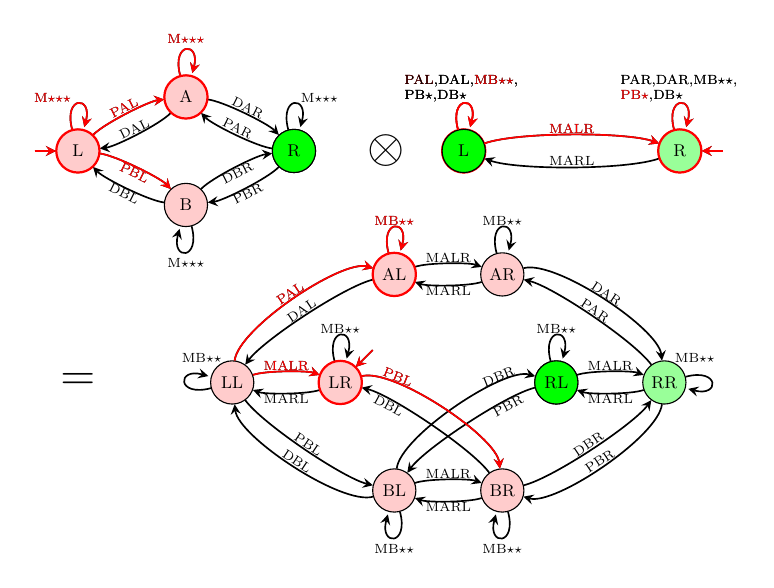
\begin{tikzpicture}[->,>=stealth,looseness=.5,,bend angle=20,scale=0.98]
  	\subpicatomicprojectionpackagesmall
	\node (otimes) at (4,0) {\LARGE $\otimes$};	
	\begin{scope}[xshift=5cm]
  	\subpicatomicprojectiontruckasmall
	\end{scope}
	\node (otimes) at (0,-3) {\LARGE $=$};	
	\begin{scope}[xshift=2cm,yshift=-3cm]
  	\subpicproductpackagetruckasmall
	\end{scope}
  \end{tikzpicture}
}


\newcommand{\picshrinkexampleone}[1][]{%
  \begin{tikzpicture}[->,>=stealth,looseness=.5,,bend angle=20,#1]
  	\vertex{0,0}{LL}
  	\vertex{2,0}{LR}
	\only<all:1-4>{\vertex{3,2}{AL}}
	\only<all:1-4>{\vertex{5,2}{AR}}
	\only<all:4>{\vertex[draw=red,thick]{3,2}{AL}}
	\only<all:4>{\vertex[draw=red,thick]{5,2}{AR}}
	\only<all:5-8>{\vertex{4,2}{A}}
	\only<all:8>{\vertex[draw=red,thick]{4,2}{A}}

	\only<all:1-6>{\vertex{3,-2}{BL}}
	\only<all:1-6>{\vertex{5,-2}{BR}}
	\only<all:6>{\vertex[draw=red,thick]{3,-2}{BL}}
	\only<all:6>{\vertex[draw=red,thick]{5,-2}{BR}}
	\only<all:7-8>{\vertex{4,-2}{B}}
	\only<all:8>{\vertex[draw=red,thick]{4,-2}{B}}
	\only<all:9->{\vertex{4,0}{I}}

	\only<all:1>{\goalvertex{6,0}{RL}}
  	\only<all:1>{\goalvertex{8,0}{RR}}
  	\only<all:2>{\goalvertex[draw=red,thick]{6,0}{RL}}
  	\only<all:2>{\goalvertex[draw=red,thick]{8,0}{RR}}
	\only<all:3->{\goalvertex{7,0}{R}}

	
	\draw[transition,->,>=stealth](2.6,0.6) -- (LR);
	\bendtransition{LL}{LR}{MALR}{}{bend left}
	\only<all:1-8>{\bendtransition{LR}{LL}{MARL}{below=-2mm}{bend left}}
	\only<all:9->{\bendtransition{LR}{LL}{MARL}{}{bend left}}
	\only<all:1-4>{\bendtransition{AL}{AR}{MALR}{}{bend left}}
	\only<all:1-4>{\bendtransition{AR}{AL}{MARL}{below=-2mm}{bend left}}
	\only<all:1-6>{\bendtransition{BL}{BR}{MALR}{}{bend left}}
	\only<all:1-6>{\bendtransition{BR}{BL}{MARL}{below=-2mm}{bend left}}
	\only<all:1-2>{\bendtransition{RL}{RR}{MALR}{}{bend left}}
	\only<all:1-2>{\bendtransition{RR}{RL}{MARL}{below=-2mm}{bend left}}
	
	\only<all:1-4>{\bendtransition{LL}{AL}{PAL}{}{bend left=50}}
	\only<all:1-4>{\bendtransition{AL}{LL}{DAL}{}{bend right}}
	\only<all:5-8>{\bendtransition{LL}{A}{PAL}{}{bend left=50}}
	\only<all:5-8>{\bendtransition{A}{LL}{DAL}{}{bend right}}
	\only<all:1-2>{\bendtransition{AR}{RR}{DAR}{}{bend left=50}}
	\only<all:1-2>{\bendtransition{RR}{AR}{PAR}{}{bend right}}
	\only<all:3-4>{\bendtransition{AR}{R}{DAR}{}{bend left=50}}
	\only<all:3-4>{\bendtransition{R}{AR}{PAR}{}{bend right}}
	\only<all:5-8>{\bendtransition{A}{R}{DAR}{}{bend left=50}}
	\only<all:5-8>{\bendtransition{R}{A}{PAR}{}{bend right}}
	\only<all:1-2>{\bendtransition{RR}{BR}{PBR}{}{bend left=50}}
	\only<all:1-2>{\bendtransition{BR}{RR}{DBR}{}{bend right}}
	\only<all:3-6>{\bendtransition{R}{BR}{PBR}{}{bend left=50}}
	\only<all:3-6>{\bendtransition{BR}{R}{DBR}{}{bend right}}
	\only<all:7-8>{\bendtransition{R}{B}{PBR}{}{bend left=50}}
	\only<all:7-8>{\bendtransition{B}{R}{DBR}{}{bend right}}
	\only<all:1-6>{\bendtransition{BL}{LL}{DBL}{}{bend left=50}}
	\only<all:1-6>{\bendtransition{LL}{BL}{PBL}{}{bend right}}
	\only<all:7-8>{\bendtransition{B}{LL}{DBL}{}{bend left=50}}
	\only<all:7-8>{\bendtransition{LL}{B}{PBL}{}{bend right}}
	
	\only<all:1-6>{\bendtransition{LR}{BR}{PBL}{near start}{bend left=50}}
	\only<all:1-6>{\bendtransition{BR}{LR}{DBL}{near end,below=-2mm}{bend right}}
	\only<all:7-8>{\bendtransition{LR}{B}{PBL}{near start}{bend left=50}}
	\only<all:7-8>{\bendtransition{B}{LR}{DBL}{near end,below=-2mm}{bend right}}
	\only<all:1-2>{\bendtransition{BL}{RL}{DBR}{near end}{bend left=50}}%
	\only<all:1-2>{\bendtransition{RL}{BL}{PBR}{near start,below=-2mm}{bend right}}%
	\only<all:3-6>{\bendtransition{BL}{R}{DBR}{near end}{bend left=50}}%
	\only<all:3-6>{\bendtransition{R}{BL}{PBR}{near start,below=-2mm}{bend right}}%
	
	\bendtransition{LL}{LL}{MB{\wildcard}{\wildcard}}{above=2mm,sloped=false,pos=.9}{loop left}
	\only<all:1-2>{\bendtransition{RR}{RR}{MB{\wildcard}{\wildcard}}{above=2mm,sloped=false,pos=.1}{loop right}}
	\only<all:1-4>{\bendtransition{AL}{AL}{MB{\wildcard}{\wildcard}}{}{loop above}}
	\only<all:1-4>{\bendtransition{AR}{AR}{MB{\wildcard}{\wildcard}}{}{loop above}}
	\only<all:5-8>{\bendtransition{A}{A}{M{\wildcard}{\wildcard}{\wildcard}}{}{loop above}}
	\bendtransition{LR}{LR}{MB{\wildcard}{\wildcard}}{}{loop above}
	\only<all:1-2>{\bendtransition{RL}{RL}{MB{\wildcard}{\wildcard}}{}{loop above}}
	\only<all:1-6>{\bendtransition{BL}{BL}{MB{\wildcard}{\wildcard}}{below=-1mm}{loop below}}
	\only<all:7-8>{\bendtransition{B}{B}{M{\wildcard}{\wildcard}{\wildcard}}{below=-1mm}{loop below}}
	\only<all:3->{\bendtransition{R}{R}{M{\wildcard}{\wildcard}{\wildcard}}{above=2mm,sloped=false}{loop right}}
	\only<all:1-6>{\bendtransition{BR}{BR}{MB{\wildcard}{\wildcard}}{below=-1mm}{loop below}}

	\only<all:9->{\bendtransition{I}{R}{D{\wildcard}R}{}{bend left}}
	\only<all:9->{\bendtransition{R}{I}{P{\wildcard}R}{}{bend left}}
	\only<all:9->{\bendtransition{I}{I}{M{\wildcard}{\wildcard}{\wildcard}}{}{loop above}}
	\only<all:9->{\bendtransition{LR}{I}{PBL}{}{bend left}}
	\only<all:9->{\bendtransition{I}{LR}{DBL}{}{bend left}}
	\only<all:9->{\bendtransition{LL}{I}{P{\wildcard}L}{}{bend right=55}}
	\only<all:9->{\bendtransition{I}{LL}{D{\wildcard}L}{below=-2mm}{bend left=80}}
  \end{tikzpicture}
}

\newcommand{\picshrinkexampleonenumberedstates}[1][]{%
  \begin{tikzpicture}[->,>=stealth,looseness=.5,,bend angle=20,#1]
        \useasboundingbox (-1.5,-3.5) rectangle (9.5,3.5);
        %% \draw (-1.5,-3.5) rectangle (9.5,3.5);
  	\numberedvertex{0,0}{LL}{0}
  	\numberedvertex{2,0}{LR}{1}
	\only<all:1-5>{\numberedvertex{3,2}{AL}{4}}
	\only<all:1-5>{\numberedvertex{5,2}{AR}{5}}
	\only<all:5>{\numberedvertex[draw=red,thick]{3,2}{AL}{4}}
	\only<all:5>{\numberedvertex[draw=red,thick]{5,2}{AR}{5}}
	\only<all:6-9>{\numberedvertex{4,2}{A}{4}}
	\only<all:9>{\numberedvertex[draw=red,thick]{4,2}{A}{4}}

	\only<all:1-7>{\numberedvertex{3,-2}{BL}{6}}
	\only<all:1-7>{\numberedvertex{5,-2}{BR}{7}}
	\only<all:7>{\numberedvertex[draw=red,thick]{3,-2}{BL}{6}}
	\only<all:7>{\numberedvertex[draw=red,thick]{5,-2}{BR}{7}}
	\only<all:8-9>{\numberedvertex{4,-2}{B}{6}}
	\only<all:9>{\numberedvertex[draw=red,thick]{4,-2}{B}{6}}
	\only<all:10-11>{\numberedvertex{4,0}{I}{4}}
        \only<all:12>{\numberedvertex{4,0}{I}{\alert{4$\mapsto$3}}}
        \only<all:13->{\numberedvertex{4,0}{I}{\alert<all:13>{3}}}

	\only<all:1-2>{\numberedgoalvertex{6,0}{RL}{2}}
  	\only<all:1-2>{\numberedgoalvertex{8,0}{RR}{3}}
  	\only<all:3>{\numberedgoalvertex[draw=red,thick]{6,0}{RL}{2}}
  	\only<all:3>{\numberedgoalvertex[draw=red,thick]{8,0}{RR}{3}}
	\only<all:4->{\numberedgoalvertex{7,0}{R}{2}}

	
	\draw[transition,->,>=stealth](2.6,0.6) -- (LR);
	\bendtransition{LL}{LR}{MALR}{}{bend left}
	\only<all:1-9>{\bendtransition{LR}{LL}{MARL}{below=-2mm}{bend left}}
	\only<all:10->{\bendtransition{LR}{LL}{MARL}{}{bend left}}
	\only<all:1-5>{\bendtransition{AL}{AR}{MALR}{}{bend left}}
	\only<all:1-5>{\bendtransition{AR}{AL}{MARL}{below=-2mm}{bend left}}
	\only<all:1-7>{\bendtransition{BL}{BR}{MALR}{}{bend left}}
	\only<all:1-7>{\bendtransition{BR}{BL}{MARL}{below=-2mm}{bend left}}
	\only<all:1-3>{\bendtransition{RL}{RR}{MALR}{}{bend left}}
	\only<all:1-3>{\bendtransition{RR}{RL}{MARL}{below=-2mm}{bend left}}
	
	\only<all:1-5>{\bendtransition{LL}{AL}{PAL}{}{bend left=50}}
	\only<all:1-5>{\bendtransition{AL}{LL}{DAL}{}{bend right}}
	\only<all:6-9>{\bendtransition{LL}{A}{PAL}{}{bend left=50}}
	\only<all:6-9>{\bendtransition{A}{LL}{DAL}{}{bend right}}
	\only<all:1-3>{\bendtransition{AR}{RR}{DAR}{}{bend left=50}}
	\only<all:1-3>{\bendtransition{RR}{AR}{PAR}{}{bend right}}
	\only<all:4-5>{\bendtransition{AR}{R}{DAR}{}{bend left=50}}
	\only<all:4-5>{\bendtransition{R}{AR}{PAR}{}{bend right}}
	\only<all:6-9>{\bendtransition{A}{R}{DAR}{}{bend left=50}}
	\only<all:6-9>{\bendtransition{R}{A}{PAR}{}{bend right}}
	\only<all:1-3>{\bendtransition{RR}{BR}{PBR}{}{bend left=50}}
	\only<all:1-3>{\bendtransition{BR}{RR}{DBR}{}{bend right}}
	\only<all:4-7>{\bendtransition{R}{BR}{PBR}{}{bend left=50}}
	\only<all:4-7>{\bendtransition{BR}{R}{DBR}{}{bend right}}
	\only<all:8-9>{\bendtransition{R}{B}{PBR}{}{bend left=50}}
	\only<all:8-9>{\bendtransition{B}{R}{DBR}{}{bend right}}
	\only<all:1-7>{\bendtransition{BL}{LL}{DBL}{}{bend left=50}}
	\only<all:1-7>{\bendtransition{LL}{BL}{PBL}{}{bend right}}
	\only<all:8-9>{\bendtransition{B}{LL}{DBL}{}{bend left=50}}
	\only<all:8-9>{\bendtransition{LL}{B}{PBL}{}{bend right}}
	
	\only<all:1-7>{\bendtransition{LR}{BR}{PBL}{near start}{bend left=50}}
	\only<all:1-7>{\bendtransition{BR}{LR}{DBL}{near end,below=-2mm}{bend right}}
	\only<all:8-9>{\bendtransition{LR}{B}{PBL}{near start}{bend left=50}}
	\only<all:8-9>{\bendtransition{B}{LR}{DBL}{near end,below=-2mm}{bend right}}
	\only<all:1-3>{\bendtransition{BL}{RL}{DBR}{near end}{bend left=50}}%
	\only<all:1-3>{\bendtransition{RL}{BL}{PBR}{near start,below=-2mm}{bend right}}%
	\only<all:4-7>{\bendtransition{BL}{R}{DBR}{near end}{bend left=50}}%
	\only<all:4-7>{\bendtransition{R}{BL}{PBR}{near start,below=-2mm}{bend right}}%
	
	\bendtransition{LL}{LL}{MB{\wildcard}{\wildcard}}{above=2mm,sloped=false,pos=.9}{loop left}
	\only<all:1-3>{\bendtransition{RR}{RR}{MB{\wildcard}{\wildcard}}{above=2mm,sloped=false,pos=.1}{loop right}}
	\only<all:1-5>{\bendtransition{AL}{AL}{MB{\wildcard}{\wildcard}}{}{loop above}}
	\only<all:1-5>{\bendtransition{AR}{AR}{MB{\wildcard}{\wildcard}}{}{loop above}}
	\only<all:6-9>{\bendtransition{A}{A}{M{\wildcard}{\wildcard}{\wildcard}}{}{loop above}}
	\bendtransition{LR}{LR}{MB{\wildcard}{\wildcard}}{}{loop above}
	\only<all:1-3>{\bendtransition{RL}{RL}{MB{\wildcard}{\wildcard}}{}{loop above}}
	\only<all:1-7>{\bendtransition{BL}{BL}{MB{\wildcard}{\wildcard}}{below=-1mm}{loop below}}
	\only<all:8-9>{\bendtransition{B}{B}{M{\wildcard}{\wildcard}{\wildcard}}{below=-1mm}{loop below}}
	\only<all:4->{\bendtransition{R}{R}{M{\wildcard}{\wildcard}{\wildcard}}{above=2mm,sloped=false}{loop right}}
	\only<all:1-7>{\bendtransition{BR}{BR}{MB{\wildcard}{\wildcard}}{below=-1mm}{loop below}}

	\only<all:10->{\bendtransition{I}{R}{D{\wildcard}R}{}{bend left}}
	\only<all:10->{\bendtransition{R}{I}{P{\wildcard}R}{}{bend left}}
	\only<all:10->{\bendtransition{I}{I}{M{\wildcard}{\wildcard}{\wildcard}}{}{loop above}}
	\only<all:10->{\bendtransition{LR}{I}{PBL}{}{bend left}}
	\only<all:10->{\bendtransition{I}{LR}{DBL}{}{bend left}}
	\only<all:10->{\bendtransition{LL}{I}{P{\wildcard}L}{}{bend right=55}}
	\only<all:10->{\bendtransition{I}{LL}{D{\wildcard}L}{below=-2mm}{bend left=80}}
  \end{tikzpicture}
}

\newcommand{\picshrinkexampleoneresult}{%
  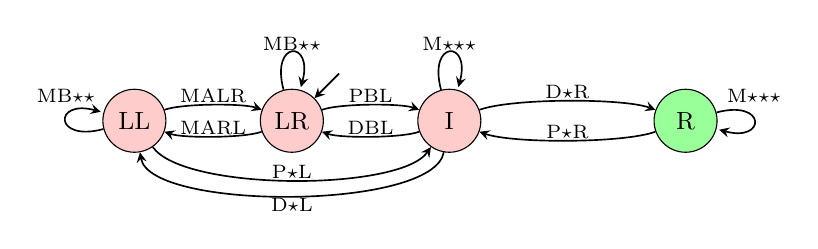
\begin{tikzpicture}[->,>=stealth,looseness=.5,,bend angle=20]
  	\vertex{0,0}{LL}
  	\vertex{2,0}{LR}
	\vertex{4,0}{I}
	\goalvertex{7,0}{R}
	
	\draw[transition,->,>=stealth](2.6,0.6) -- (LR);
	\bendtransition{LL}{LR}{MALR}{}{bend left}
	\bendtransition{LR}{LL}{MARL}{}{bend left}
	\bendtransition{LL}{LL}{MB{\wildcard}{\wildcard}}{above=2mm,sloped=false}{loop left}
	\bendtransition{LR}{LR}{MB{\wildcard}{\wildcard}}{}{loop above}
	\bendtransition{R}{R}{M{\wildcard}{\wildcard}{\wildcard}}{above=2mm,sloped=false}{loop right}
	\bendtransition{I}{R}{D{\wildcard}R}{}{bend left}
	\bendtransition{R}{I}{P{\wildcard}R}{}{bend left}
	\bendtransition{I}{I}{M{\wildcard}{\wildcard}{\wildcard}}{}{loop above}
	\bendtransition{LR}{I}{PBL}{}{bend left}
	\bendtransition{I}{LR}{DBL}{}{bend left}
	\bendtransition{LL}{I}{P{\wildcard}L}{}{bend right=55}
	\bendtransition{I}{LL}{D{\wildcard}L}{below=-2mm}{bend left=80}
  \end{tikzpicture}
}

\newcommand{\picshrinkexampleoneresultdifferent}{%
  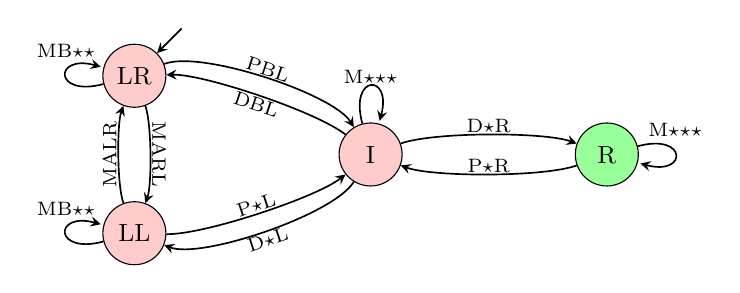
\begin{tikzpicture}[->,>=stealth,looseness=.5,,bend angle=20]
  	\vertex{0,-1}{LL}
  	\vertex{0,1}{LR}
	\vertex{3,0}{I}
	\goalvertex{6,0}{R}
	
	\draw[transition,->,>=stealth](0.6,1.6) -- (LR);
	\bendtransition{LL}{LR}{MALR}{}{bend left}
	\bendtransition{LR}{LL}{MARL}{}{bend left}
	\bendtransition{LL}{LL}{MB{\wildcard}{\wildcard}}{above=2mm,sloped=false}{loop left}
	\bendtransition{LR}{LR}{MB{\wildcard}{\wildcard}}{above=2mm,sloped=false}{loop left}
	\bendtransition{R}{R}{M{\wildcard}{\wildcard}{\wildcard}}{above=2mm,sloped=false}{loop right}
	\bendtransition{I}{R}{D{\wildcard}R}{}{bend left}
	\bendtransition{R}{I}{P{\wildcard}R}{}{bend left}
	\bendtransition{I}{I}{M{\wildcard}{\wildcard}{\wildcard}}{}{loop above}
	\bendtransition{LR}{I}{PBL}{}{bend left=40}
	\bendtransition{I}{LR}{DBL}{below=-2mm}{bend right}
	\bendtransition{LL}{I}{P{\wildcard}L}{}{bend right}
	\bendtransition{I}{LL}{D{\wildcard}L}{below=-2mm}{bend left=40}
  \end{tikzpicture}
}

\newcommand{\picproductfinal}[1][]{%
  \begin{tikzpicture}[->,>=stealth,looseness=.5,,bend angle=20,#1]
  	\vertex{-.5,2.5}{LRL}
  	\vertex{1,1.5}{LRR}
  	\vertex{-.5,-1.5}{LLL}
  	\vertex{1,-2.5}{LLR}
  	\vertex{3,0.5}{IL}
  	\vertex{4.5,-.5}{IR}
  	\goalvertex{6.5,0.5}{RL}
  	\goalvertex{8,-.5}{RR}

	\draw[transition,->,>=stealth](1.6,1.1) -- (LRR);

	\bendtransition{LRL}{LRR}{MBLR}{below=-2mm}{bend left}
	\bendtransition{LRR}{LRL}{MBRL}{below=-2mm}{bend left}
	\bendtransition{LLL}{LLR}{MBLR}{below=-2mm}{bend left}
	\bendtransition{LLR}{LLL}{MBRL}{below=-2mm}{bend left}
	\bendtransition{IL}{IR}{MBLR}{}{bend left}
	\bendtransition{IR}{IL}{MBRL}{}{bend left}
	\bendtransition{RL}{RR}{MBLR}{}{bend left}
	\bendtransition{RR}{RL}{MBRL}{}{bend left}

	\bendtransition{IL}{RL}{DAR}{}{bend left=40}
	\bendtransition{RL}{IL}{PAR}{below=-2mm}{bend right}
	\bendtransition{IR}{RR}{D{\wildcard}R}{}{bend right}
	\bendtransition{RR}{IR}{P{\wildcard}R}{below=-2mm}{bend left=40}
	\bendtransition{LLL}{IL}{P{\wildcard}L}{near end,below=-2mm}{bend left}
	\bendtransition{IL}{LLL}{D{\wildcard}L}{below=-2mm,near start}{bend left}
	\bendtransition{LLR}{IR}{PAL}{}{bend right}
	\bendtransition{IR}{LLR}{DAL}{below=-2mm}{bend left=40}

	\bendtransition{LLL}{LRL}{MALR}{}{bend left=50}
	\bendtransition{LRL}{LLL}{MARL}{rotate=180,below=0mm}{bend right}
	\bendtransition{LLR}{LRR}{MALR}{near end}{bend left}
	\bendtransition{LRR}{LLR}{MARL}{rotate=180,above=-2mm,near start}{bend left}

	\bendtransition{LRL}{IL}{PBL}{}{bend left=60}
	\bendtransition{IL}{LRL}{DBL}{}{bend right=30}
	\bendtransition{IL}{IL}{MA{\wildcard}{\wildcard}}{below=-1mm}{loop below}
	\bendtransition{IR}{IR}{MA{\wildcard}{\wildcard}}{below=-1mm}{loop below}
	\bendtransition{RR}{RR}{MA{\wildcard}{\wildcard}}{below=-1mm}{loop below}
	\bendtransition{RL}{RL}{MA{\wildcard}{\wildcard}}{}{loop above}
  \end{tikzpicture}
}

\newcommand{\picshrinkexampletworesult}{%
  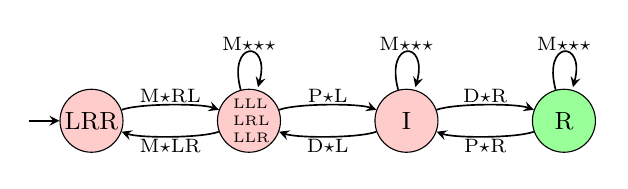
\begin{tikzpicture}[->,>=stealth,looseness=.5,,bend angle=20]
  	\vertex{0,0}{LRR}
    \node[vertex interior] at (2,0) (LLL) {};
    \node[vertex border] at (2,0) {\parbox{4mm}{\tiny LLL\\LRL\\LLR}};
	\vertex{4,0}{I}
	\goalvertex{6,0}{R}
	
	\draw[transition,->,>=stealth](-0.8,0) -- (LRR);
	\bendtransition{I}{I}{M{\wildcard}{\wildcard}{\wildcard}}{}{loop above}
	\bendtransition{R}{R}{M{\wildcard}{\wildcard}{\wildcard}}{}{loop above}
	\bendtransition{LLL}{LLL}{M{\wildcard}{\wildcard}{\wildcard}}{}{loop above}

	\bendtransition{LRR}{LLL}{M{\wildcard}RL}{}{bend left}
	\bendtransition{LLL}{LRR}{M{\wildcard}LR}{below=-2mm}{bend left}
	\bendtransition{LLL}{I}{P{\wildcard}L}{}{bend left}
	\bendtransition{I}{LLL}{D{\wildcard}L}{below=-2mm}{bend left}
	\bendtransition{I}{R}{D{\wildcard}R}{}{bend left}
	\bendtransition{R}{I}{P{\wildcard}R}{below=-2mm}{bend left}
  \end{tikzpicture}
}
